

\documentclass[11pt,technote]{IEEEtran}

\usepackage{geometry}
\geometry{hmargin=2cm,vmargin=2cm}

\usepackage{algorithm2e}
\usepackage{graphicx}
\usepackage{tabularx}
\usepackage{fourier}
\usepackage{hyperref}
\usepackage{multirow}
\usepackage{caption}
\usepackage{subcaption}
\usepackage{amsmath}
\usepackage{float}



\usepackage{rotating}	%% introduce sideways env
\usepackage{tikz}
\usepackage{amssymb}

%% Public TikZ libraries
\usetikzlibrary{positioning}
\usetikzlibrary{shapes}
\usetikzlibrary{calc}


\usetikzlibrary{arrows}			%% Include regular arrows
\usetikzlibrary{arrows.meta}	
%\usepgflibrary{myarrows.new}		%% Include custom arrows


\tikzset{XOR/.style={draw,
		circle,
		append after command={
			[shorten >=\pgflinewidth, shorten <=\pgflinewidth,]
			(\tikzlastnode.north) edge[] (\tikzlastnode.south)
			(\tikzlastnode.east) edge[] (\tikzlastnode.west)
		},
	},
}

\tikzset{edge/.style={
		-latex new, 
		arrow head=6pt, 
		%						thick
	},
}

\tikzset{line/.style={
		%						thick,
		draw, 
		%						-latex',
		shorten <=1bp,
		shorten >=1bp,
	}
}

\newcommand{\AEheight}{0.75cm}
\newcommand{\AEwidth}{1.5cm}

\tikzset{AE_P/.style={
		rectangle,
		thick,
		draw,
		fill=yellow!20,
		inner sep = 0pt,
		outer sep = 0pt,
		text width=1cm, 
		minimum height=4.5cm,
		text centered,
		%		anchor=north,
	}	
}

\tikzset{AE_vert/.style={
		rectangle,
		thick,
		draw,
		fill=blue!20,
		inner sep = 0pt,
		outer sep = 0pt,
		text width=\AEheight, 
		minimum height=\AEwidth,
		text centered,
		%		anchor=north,
	}
}

\tikzset{AE_msg/.style={
		rectangle,
		thick,
		draw,
		fill=blue!20,
		inner sep = 0pt,
		outer sep = 0pt,
		text width=\AEwidth,
		minimum height=\AEheight,
		text centered,
		%		anchor=north,
	}
}

\tikzset{AE_ctx/.style={
		rectangle,
		thick,
		draw,
		fill=green!20,
		inner sep = 0pt,
		outer sep = 0pt,
		text width=\AEwidth, 
		minimum height=\AEheight,
		text centered,
		%		anchor=north,
	}
}

\tikzset{AE_key/.style={
		rectangle,
		thick,
		draw,
		fill=red!20,
		inner sep = 0pt,
		outer sep = 0pt,
		text width=\AEwidth, 
		minimum height=\AEheight,
		text centered,
		%		anchor=north,
	}
}

\tikzset{AE_tag/.style={
		rectangle,
		thick,
		draw,
		fill=green!20,
		inner sep = 0pt,
		outer sep = 0pt,
		text width=\AEwidth, 
		minimum height=\AEheight,
		text centered,
		%		anchor=north,
	}
}




\usepackage{xcolor}
\usepackage{listings}

\definecolor{mGreen}{rgb}{0,0.6,0}
\definecolor{mGray}{rgb}{0.5,0.5,0.5}
\definecolor{mPurple}{rgb}{0.58,0,0.82}
\definecolor{backgroundColour}{rgb}{0.95,0.95,0.92}

\lstdefinestyle{CStyle}{
	backgroundcolor=\color{backgroundColour},   
	commentstyle=\color{mGreen},
	keywordstyle=\color{magenta},
	numberstyle=\tiny\color{mGray},
	stringstyle=\color{mPurple},
	basicstyle=\tiny,
	breakatwhitespace=false,         
	breaklines=true,                 
	captionpos=b,                    
	keepspaces=true,                 
	numbers=left,                    
	numbersep=5pt,                  
	showspaces=false,                
	showstringspaces=false,
	showtabs=false,                  
	tabsize=2,
	language=C
}

\author{
	Alexane Boldo\\
	Internship from 19/05/2025 to 11/07/2025\\
	Supervisor: Hélène Le Bouder\\
	OCIF, IRISA
}

\title{Side-channel attacks on Ascon's S-box}
\date{}

%\counterwithout{section}{chapter}
%\counterwithout{figure}{chapter}

\begin{document}
	\maketitle
	
	% Un petit résumé
	\begin{abstract}
		Though side-channel attacks on the National Institute of Standards and Technology winner Ascon have succeeded, simple correlation power analysis attacks targeting the S-box have failed. However, some of its properties can give more information on potential attacks, like the direction of computation or its relatively simple equations. Therefore, this article is interested in finding if those weaknesses can lead to an attack, using multiple traces of the power consumption captured by a ChipWhisperer and analyzing their correlation with the output of the S-box. The theorized attack uses a link between the key and the output, and it was found that computing seems to leak better than writing in the register. However, we were unable to use the relatively easy equations from the S-box to find weaknesses, even while controlling the nonces by attacking the decryption phase.
	\end{abstract}
	
	%\tableofcontents
	
	\section{Introduction}
	Though mathematically secure, cryptographic algorithms can still be broken. Indeed, leakages happen during the computation of the encryption, which can be observed and analyzed to figure out the key. Such leakages can be the computation time, the power consumption, or the electromagnetic radiations and can lead to attacks recovering the key, called side-channel attacks (SCA). Therefore, a whole field of cybersecurity consists of analyzing which computations leak the most data.\\
	This article focuses on Ascon \cite{ascon}, the winner of the National Institute of Standards and Technology (NIST) competition for Authenticated Encryption with Associated Data (AEAD), which became the standard for lightweight cryptography \cite{norme}. Multiple attacks \cite{cpa_lin,dl_cpa} based on Correlation Power Analysis (CPA) \cite{cpa_aes} have already been performed and analyzed \cite{cpa_analysis} to find a stronger implementation of Ascon, using masking to render SCA harder.\\
	However, to our knowledge, no CPA attack on the non-linear layer of the permutation were successful, although such permutations are known to provide leakage. Furthermore, an analysis provided by Sarry\cite{these} deducts equations to link the output of this layer to the secret key.\\
	Therefore, this article uses a CPA in order to determine where exactly the leakage is the clearer, by attacking the output of the substitution layer of the first-round of the permutation. The goal is to provide an analysis finding the best path to attack it.\\
	This paper first describes Ascon-AEAD then the methodology used to attack it. Next, it presents the best choices for the CPA attack after a small presentation of its concept. Lastly, Sarry's equations \cite{these} are used to try an attack, and its failure is analyzed.
	
	\section{Description of Ascon}
	\subsection{Generalities}
	This paper focuses on Ascon-AEAD as described in the norm \cite{norme}. This paper especially focuses on the decryption phase to use the leaks in order to recover the key.
	
	\begin{algorithm}[h]
		\KwData{128-bit key $K$ and nonce $N$, associated data $A$, ciphertext $C$ and 128-bit tag $T$}
		\KwResult{checks authentication with $T$, if it is authenticated returns plaintext $P$ otherwise returns fail}
	\end{algorithm}
	
	This algorithm uses a 320-bit state, divided into 5 64-bit words and modified through 4 phases: the initialization, the associated data process, the ciphertext process, and the finalization. IV is a known constant given in the norm \cite{norme}, and in the following, this paper refers to the rate as $r=128$.
	
	
	\subsection{Ascon's permutation}	\label{perm}	
	This algorithm uses a permutation $p = p_L \circ p_S \circ p_C$, which is used at all phases of the encryption or decryption and is the target of the attack. Each notation \ref{notations} is described in more detail in the annex. This permutation is itself divided into three layers: the constant-addition layer $p_C$ that adds to the end of the third word an 8-bit round-dependent constant; the substitution layer $p_S$, which is a 5-bit S-box taking the $j^{th}$ bit of each word; and the linear-diffusion layer $p_L$ rotating each word to provide diffusion to the cipher where $\forall i \in \llbracket 1;5 \rrbracket, S_i \leftarrow \Sigma_i(S_i)$:
	
	\begin{gather*}
		\Sigma_0(S_0) = S_0 \oplus (S_0 >>> 19) \oplus (S_0 >>> 28)\\
		\Sigma_1(S_1) = S_1 \oplus (S_1 >>> 61) \oplus (S_1 >>> 39)\\
		\Sigma_2(S_2) = S_2 \oplus (S_2 >>> \;  1) \oplus (S_2 >>> \; 6)\\
		\Sigma_3(S_3) = S_3 \oplus (S_3 >>> 10) \oplus (S_3 >>> 17)\\
		\Sigma_4(S_4) = S_4 \oplus (S_4 >>> \; 7) \oplus (S_4 >>> 41)\\
	\end{gather*}
	
	The substitution layer is the one attacked in this article. It is a non-linear permutation, providing confusion to the cipher and computing each column of the state separately, using the circuit \ref{circuit_sbox}. Formally, let's write $\sigma=p_S(S)$\\
	The substitution layer computes for each $j \in \llbracket 1;64 \rrbracket$:
	$$(\sigma_0^j,\sigma_1^j,\sigma_2^j,\sigma_3^j,\sigma_4^j) = S-box(S_0^j,S_1^j,S_2^j,S_3^j,S_4^j)$$
	
	\begin{figure}[H]
		\centering
		\includegraphics[scale=0.4]{img_files/circuit}
		\caption{Circuit to compute the S-box, from \cite{norme}}
		\label{circuit_sbox}
	\end{figure}
	
	
	\subsection{Ascon-AEAD's algorithm}
	Each step of the algorithm is described here, and the complete figure from \cite{cours_crypto} for the encryption can be found in the annex \ref{fig:enc}.
	
	\begin{enumerate}
		\item Initialization: state creation and modification
		$$S \leftarrow p^{a}( \underbrace{IV}_{S_0}||\underbrace{K}_{S_1,S_2}||\underbrace{n}_{S_3,S_4})$$
		\resizebox{80pt}{80pt}{
	
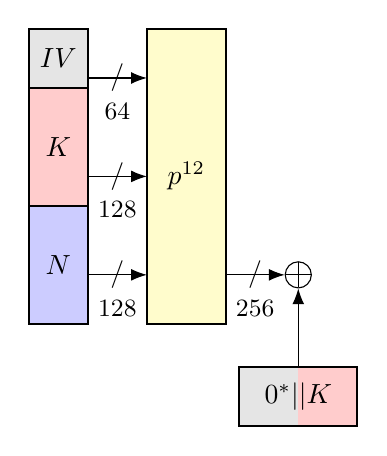
\begin{tikzpicture}[node distance = 1cm and 0.75cm]

% init
\node[AE_P, minimum height = 3.75cm] (pi) {$p^{12}$};

\node[AE_vert, fill = gray!20, left = of pi.north west, anchor = north east, minimum height = 0.75cm] (iv) {$IV$}; 

\node[AE_vert, fill = red!20, anchor = north] (k)  at (iv.south) {$K$}; 
\node[AE_vert, fill = blue!20, left = of pi.south west, anchor = south east] (n) {$N$}; 

\coordinate (helpsouth) at ($(pi.south east)!1/6!(pi.north east)$);
\coordinate (helpnorth) at ($(pi.south east)!5/6!(pi.north east)$);

\draw[-{Latex[length=2mm]}] (iv.east|-helpnorth) -> (helpnorth-|pi.west) node[midway] {$/$} node[midway, below=0.2cm] {\small $64$};
\draw[-{Latex[length=2mm]}] (k.east|-pi.west) -- (pi.west) node[midway] {$/$} node[midway, below=0.2cm] {\small $128$};
\draw[-{Latex[length=2mm]}] (n.east|-helpsouth) -- (helpsouth-|pi.west) node[midway] {$/$} node[midway, below=0.2cm] {\small $128$};

\node[XOR, right = of pi.east|-helpsouth] (xkinit) {};
\node[AE_key, anchor = west, below = of xkinit, path picture={
      \fill[gray!20] (path picture bounding box.north) rectangle (path picture bounding box.south west);
    }] (kinit) {$0^* || K$};

\draw[-{Latex[length=2mm]}] (pi.east|-helpsouth) -- (xkinit) node[midway] {$/$} node[midway, below=0.2cm] {\small $256$}; 
\draw[-{Latex[length=2mm]}] (kinit.north-|xkinit) -- (xkinit); 

% separations


\end{tikzpicture}
}
		\item Associated data process: for the authentication of $A$, updates $S$ using $A=(A_1||...||A_s)$ parsed into blocks of $r$-bits, except for the last of size $|A|\%r$\\
		\resizebox{160pt}{85pt}{
	
\begin{tikzpicture}[node distance = 1cm and 0.75cm]


% 1er tour AD

\node[XOR, right = of kinit.east|-helpnorth] (xa1) {};

\node[AE_msg, above = of xa1] (a1) {$A_1$};

\draw[-{Latex[length=2mm]}] (a1) -- (xa1) node[midway] {$/$} node[midway, left=0.2cm] {\small $128$};
\draw[line] (pi.east|-xa1) -- (helpnorth-|xkinit) node[midway] {$/$} node[midway, below=0.2cm] {\small $128$};
\draw[-{Latex[length=2mm]}] (pi.east|-xa1)  -- (xa1);


% 2er tour AD


\node[AE_P, minimum height = 3.75cm, right = of xa1|-pi] (pa1) {$p^{8}$};

\draw[-{Latex[length=2mm]}] (xkinit) -- (pa1.west|-xkinit);
\draw[-{Latex[length=2mm]}] (xa1) -- (pa1.west|-xa1);

\node[right = of pa1.east|-helpnorth, inner sep = 10pt] (cdotnortha) {$\cdots$};
\node[right = of pa1.east|-helpsouth, inner sep = 10pt] (cdotsoutha) {$\cdots$};

\node[XOR, right = of cdotnortha] (xa2) {};
\node[AE_msg, above = of xa2, path picture={
      \fill[gray!20] (path picture bounding box.north) rectangle (path picture bounding box.south east);
    }] (a2) {$A_{s}||10^*$};


\draw[line] (pa1.east|-cdotnortha) -- (cdotnortha);
\draw[line] (pa1.east|-cdotsoutha) -- (cdotsoutha);
\draw[-{Latex[length=2mm]}] (cdotnortha) -- (xa2);
\draw[-{Latex[length=2mm]}] (a2) -- (xa2) node[midway] {$/$} node[midway, left=0.2cm] {\small $128$};


% fin AD

\node[AE_P, minimum height = 3.75cm, right = of xa2|-pa1] (pa2) {$p^{8}$};

\node[XOR, right = of pa2.east|-helpsouth] (xdom) {};
\node[AE_key, fill = gray!20, below = of xdom] (dom) {$0^*1$};

\draw[-{Latex[length=2mm]}] (xa2) -- (pa2.west|-xa2);
\draw[-{Latex[length=2mm]}] (cdotsoutha) -- (pa2.west|-helpsouth);

\draw[-{Latex[length=2mm]}] (pa2.east|-xdom) -- (xdom);
\draw[-{Latex[length=2mm]}] (dom.north-|xdom) -- (xdom);


% separations


\end{tikzpicture}
}
		\item Ciphertext process: $C = (C_1 || ... || C_t)$ is parsed with $C_i$ of size $r$ except for $C_t$ of size $l=|C| \% r$. Each block of the ciphertext is then XORed to $S$ to find the associated plaintext, and then the beginning of $S$ is replaced by this ciphertext block:\\
		\resizebox{220pt}{75pt}{
	
\begin{tikzpicture}[node distance = 1cm and 0.75cm]

% 1er tour chiffrement

\node[XOR, right = of dom.east|-helpnorth] (x1) {};
\node[AE_ctx, above = of x1] (m1) {$P_1$};
\node[AE_msg, right = of m1] (c1) {$C_1$};

\draw[-{Latex[length=2mm]}] (pa2.east|-x1) -- (x1);
\draw[-{Latex[length=2mm]}] (x1) -- (m1) node[midway] {$/$} node[midway, left=0.2cm] {\small $128$};
\draw[-{Latex[length=2mm]}] (c1) |- (x1) node[near end] {$/$} node[near end, above=0.2cm] {\small $128$};

\node at (x1-|c1) {$\bullet$};

% 2e tour chiffrement

\node[AE_P, minimum height = 3.75cm, right = of c1|-pa2] (p1) {$p^{8}$};

\draw[-{Latex[length=2mm]}] (x1) -- (x1-|p1.west);
\draw[-{Latex[length=2mm]}] (xdom) -- (p1.west|-helpsouth);

\node[right = of p1.east|-helpnorth, inner sep = 10pt] (cdotnorth) {$\cdots$};
\node[right = of p1.east|-helpsouth, inner sep = 10pt] (cdotsouth) {$\cdots$};

\node[XOR, right = of cdotnorth] (x2) {};
\node[AE_ctx, above = of x2] (m2) {$P_{t-1}$};
\node[AE_msg, right = of m2] (c2) {$C_{t-1}$};


\draw[line] (p1.east|-cdotnorth) -- (cdotnorth);
\draw[line] (p1.east|-cdotsouth) -- (cdotsouth);

\draw[-{Latex[length=2mm]}] (cdotnorth) -- (x2);
\draw[-{Latex[length=2mm]}] (x2) -- (m2) node[midway] {$/$} node[midway, left=0.2cm] {\small $128$};
\draw[-{Latex[length=2mm]}] (c2) |- (x2) node[near end] {$/$} node[near end, above=0.2cm] {\small $128$};

\node at (x2-|c2) {$\bullet$};


% fin chiffrement

\node[AE_P, minimum height = 3.75cm, right = of c2|-p1] (p2) {$p^{8}$};

\draw[-{Latex[length=2mm]}] (x2) -- (x2-|p2.west);
\draw[-{Latex[length=2mm]}] (cdotsouth) -- (p2.west|-cdotsouth);

\node[XOR, right = of p2.east|-x1] (x3) {};
\node[XOR, below = of x3] (x4) {};
\node[AE_ctx, above = of x3, text width = 0.75cm] (m3) {$P_{t}$};
\node[AE_msg, right = of m3, path picture={
      \fill[gray!20] (path picture bounding box.north) rectangle (path picture bounding box.south east);
    }] (c3) {$C_{t}$};
\node[AE_key, fill = gray!20, below = of x4] (dom) {$10^*$};

\draw[-{Latex[length=2mm]}] (p2.east|-x3) -- (x3);
\draw[-{Latex[length=2mm]}] (x3) -- (m3) node[midway] {$/$} node[midway, left=0.2cm] {\small $l$};
\draw[-{Latex[length=2mm]}] (c3) |- (x3) node[near end] {$/$} node[near end, above=0.2cm] {\small $l$};
\draw[-{Latex[length=2mm]}] (p2.east|-x4) -- (x4)node[midway] {$/$} node[midway, above=0.2cm] {\scriptsize $128-l$};
\draw[-{Latex[length=2mm]}] (dom) -- (x4);

\node at (x3-|c3) {$\bullet$};

\end{tikzpicture}
}
		\item Finalization: computes the tag thanks to the key and the state\\
		\resizebox{100pt}{75pt}{
	
\begin{tikzpicture}[node distance = 1cm and 0.75cm]
% finalisation

\node[XOR, right = of c3.east|-helpsouth] (xkf) {};

\node[AE_P, minimum height = 3.75cm, right = of xkf.east|-p2] (pf) {$p^{12}$};

\node[AE_key, below = of xkf, path picture={
      \fill[gray!20] (path picture bounding box.north) rectangle (path picture bounding box.south east);
    }] (kf) {$K||0^*$};

\draw[-{Latex[length=2mm]}] (x3) -- (x3-|pf.west);
\draw[-{Latex[length=2mm]}] (x4) -- (x4-|pf.west);
\draw[-{Latex[length=2mm]}] (p2.east|-xkf) -- (xkf);
\draw[-{Latex[length=2mm]}] (xkf|-kf.north) -- (xkf);
\draw[-{Latex[length=2mm]}] (xkf) -- (xkf-|pf.west);

\node[XOR, right = of pf.east|-xkf] (xt) {};
\node[AE_key, below = of xt] (kt) {$K$};
\node[AE_tag] at (c3-|xt) (t) {$T'$};

\draw[-{Latex[length=2mm]}] (pf.east|-xt) -- (xt) node[midway] {$/$} node[midway, below=0.2cm] {\small $128$};
\draw[-{Latex[length=2mm]}] (kt) -- (xt);
\draw[-{Latex[length=2mm]}] (xt) -- (t);

\end{tikzpicture}
}\\
		If $T'= T$, returns $P \leftarrow P_1 || ... || P_t$, otherwise returns \verb|fail|
	\end{enumerate}
	
	\section{Methodology}
	We implemented our version of Ascon, given in this repository\footnote{\url{https://github.com/ABo-projets/Stage_L3}} to visualize the possible implementation weaknesses, which is later compared to the reference implementation\footnote{\url{https://github.com/ascon/ascon-c/blob/main/crypto\_aead/asconaead128/ref}} from the authors of Ascon \cite{ascon}. Our version has the advantage to be able to follow other constants than those given by the norm.
	
	In order to attack the implementations, a ChipWhisperer-Lite board with an XMEGA target microcontroller (CW1173) is used to capture the power consumption during the execution of the decryption, as it gives clearer traces than in real-life scenarios.
	
	\begin{figure}[h]
		\includegraphics[width=0.5\textwidth]{img_files/cwlite_basic1}
		\caption{ChipWhisperer from \cite{cwdoc}}
		\label{fig:cw}
	\end{figure}
	
	To facilitate the capture, triggers were added in the first round of the permutation, during the initialization stage, in order to start the recording of the power consumption.
	
	10K traces with a fixed key and variable nonces, 10K traces with variable keys and nonces, 10K traces with variable keys and a fixed nonce all during the $p_S$ layer were recorded on both the reference implementation and our own. The following section explains these choices.
	
	\section{Observations for CPA attacks}
	\subsection{Correlation Power Analysis (CPA) definition}
	Correlation Power Analysis\cite{cpa_aes} is a type of attack using the recording of multiple traces of the execution of a known cryptographic algorithm to recover the private key. It can be blind (the attacker knows neither the plaintext nor the ciphertext) or not. It is often based on the divide-and-conquer approach, where the attacker recovers the key portion-by-portion (often byte-by-byte or bit-by-bit). The following explanation takes the notations used in the course \cite{cours}.
	
	\begin{enumerate}
		\item \textbf{Campaign:}
		\begin{itemize}
			\item Let's first define the target $k$ that will take all its possible values (e.g., for one byte of the key, its 256 values)
			\item Then the first step is to compute multiple traces of the targeted algorithm to gain observables (e.g., the plaintext and the power consumption as a function of time)
			\item Find an attack path, i.e., a relation between observables and the target: $\mathcal{R}(k,O_S) = O_R$. It depends on physical functions, called leak functions, and cannot be computed
		\end{itemize}
		\item \textbf{Prediction:} Because the exact leak functions cannot be computed, the attacker has to find a model to approximate it (e.g., the Hamming Weight (HW) of the byte for the power consumption, as the consumption of writing in a register depends on whether it is a 1 or a 0 that is written), it gives a new relation model, called a theoretical attack path: $\mathcal{R}_m(k,O_S) = P_{m,k}$
		\item \textbf{Confrontation:} The attacker has to find a distinguisher, i.e., a statistical function that puts a hypothesis $k_d$ upfront of the others by confronting $O_R$ and $P_{m,k}$ (e.g., the Pearson correlation between the vector of HW and the power consumptions, at each timestamp $t$). This also gives points of interest, i.e., timestamps where the target is used.
	\end{enumerate}
	
	This attack is well established on the previous encryption standard AES \cite{cpa_aes,aes} by attacking the S-box; however in Ascon the S-box is computed vertically and not horizontally, whereas the results are written in the words, therefore horizontally.
	
	\begin{figure}[h]
		\centering
		\begin{subfigure}{.18\textwidth}
			\centering
			\includegraphics[width=1\linewidth]{img_files/sbox_computation}
			\caption{Computing}
			\label{fig:comp}
		\end{subfigure}
		\begin{subfigure}{.22\textwidth}
			\centering
			\includegraphics[width=.8\linewidth]{img_files/sbox_writing}
			\caption{Writing in the register}
			\label{fig:writ}
		\end{subfigure}
		\caption{Comparison of the direction for computing the S-box and writing in the register for the first byte of the five words}
		\label{fig:direction}
	\end{figure}
	
	Therefore it is pertinent to wonder, like Sarry in \cite{these}, whether the leak is horizontal or vertical, in order to determine if the S-box leaks because of the computation or of the writing in the register and to find better strategies of masking. Hereafter, this article refers to attacks on one byte of the last word of the state as horizontal attacks and to the ones on the concatenation of the 5 bits at position $j$ on each word of the state as vertical attacks.
	
	\subsection{Choosing a theoretical attack path and a distinguisher} \label{choice}
	\subsubsection{Horizontal attack on the S-box}
	In this part, the traces used are those measured on our implementation, with variable keys and a fixed nonce, in order to see what functions show the most influence from the key.
	
	The goal is to see if there is an adequate distinguisher for the key hypothesis, using the HW of the first horizontal byte. Two statistical functions seem promising: the Pearson correlation, usually used in CPA attacks, which failed to conclude for more than 40K traces in \cite{dl_cpa}, and the mutual information.
	
	\begin{figure}[h]
		\centering
		\includegraphics[scale=0.4]{img_files/horizontal_one_byte}
		\caption{Normalized mutual information between the power consumption and the Hamming weight or the value of the first byte of $S_4$}
		\label{hHW&val}
	\end{figure}
	
	In the graph \ref{hHW&val}, there are a few points of interest that seem to show an influence from the key on the power consumption on a few instances, which is a good sign to be able to find the key later. To visualize how the points of interest for each byte correlate, the graph \ref{hHW8_zoom} shows that the use of each byte of key is successive, which is logical. 
	
	\begin{figure}[h]
		\centering
		\includegraphics[scale=0.4]{img_files/hHW_8_bytes_zoom}
		\caption{Mutual information between power consumption and Hamming weight of each of the 8 bytes}
		\label{hHW8_zoom}
	\end{figure}
	
	\begin{figure}[h]
		\centering
		\includegraphics[scale=0.4]{img_files/comp_ref_hHW}
		\caption{Mutual information between power consumption and horizontal Hamming Weight on the reference implementation and on our own}
		\label{compref}
	\end{figure}
	
	To check if our implementation is worse than the reference one, the graph \ref{compref} is useful and shows that both of them have clear leaks. However, these leaks don't happen at the same time, since the S-box is not written exactly the same. 
	
	\begin{figure}[H]
		\centering
		\includegraphics[scale=0.4]{img_files/corr_vs_MI_hHW}
		\caption{Normalized mutual information and absolute Pearson correlation for a horizontal attack on the reference implementation}
		\label{corvsMI}
	\end{figure}
	
	Let's now compare the mutual information with the Pearson correlation. In the graph \ref{corvsMI}, a reassuring observation is that points of interest are the same no matter the distinguisher. Furthermore, though the absolute value is greater for the Pearson correlation, points of interest appear slightly clearer after normalization with the mutual information, which can help on the attack.
	
	\subsubsection{Vertical attack on the S-box}
	First, let's use the same traces as before and compare to see if there is an adequate distinguisher using the HW of the first output of the S-box.
	
	\begin{figure}[h!]
		\centering
		\includegraphics[scale=0.4]{img_files/vertical_one_bit}
		\caption{Mutual information between power consumption and Hamming weight of the concatenation of the first bit of each of the word of $S$ and its value}
		\label{vHW}
	\end{figure}
	
	From the graph \ref{vHW}, it seems that there are also vertical leaks, which are fewer in Hamming weight than in value, which probably includes false ones. Furthermore, studying variable nonces also illustrates the leaks, which are, however, logically more noisy with variable nonces (see in annex \ref{vHW&val}).
	
	Finally, let's compare horizontal and vertical leaks with graph \ref{hvval}. Counterintuitively, horizontal and vertical points of interest seem to coincide, which refutes the hypothesis that there is first a leak because of the computation and then another one because of writing in the register. A possible explanation would be that the mutual information is induced by the value of the bit that is both there horizontally and vertically, which could explain why correlations and mutual information are so low. However, the vertical leaks seem to be clearer, which seems to indicate that the computation leaks a lot, and it gives the attacker a clearer theoretical attack path. Furthermore, the chosen distinguisher for the following analysis is the mutual information, which looks slightly clearer.
	
	\begin{figure}[h]
		\centering
		\includegraphics[scale=0.4]{img_files/h_and_v_one_byte}
		\caption{Normalized mutual information for the horizontal and vertical Hamming weight}
		\label{hvval}
	\end{figure}
	
	\subsection{Working CPA attack with another attack path}
	Let's note that there is a working simple CPA attack, as proven by Daemen et al. in \cite{cpa_lin}. The idea is to first put the trigger before the linear-diffusion layer then have for key hypothesis the three bits of the key, which are XORed to have the output $S_0^0$, and simplifying equations thanks to their observations.
	%		
	%		\begin{figure}[h]
		%			\centering
		%			\includegraphics[scale=0.3]{img_files/graph_daemen}
		%			\caption{Absolute Pearson correlation between the output of $S_0^0$ and the power consumption as a function of time for each hypothesis for $(k_0,k_{36},k_{45})$}
		%			\label{graphs}
		%		\end{figure}
	%		
	%		This graph \ref{graphs} allows to see a key providing a clear better correlation than any other: this is the right key, and in the same time the point of interest is shown clearly.\\
	%		We were able to reproduce the experiment and recover the entire key.
	%		
	
	\section{Using equations binding the input and output of the S-box}
	\subsection{Description of the equation} \label{sec_equ}
	Sarry \cite{these} describes in his thesis equations linking the output of the S-box to the value of the key, depending on the value of the nonce and of the IV \ref{link_k_s4}. These equations are described in the annex \ref{equations}.
	
	\begin{figure}[h]
		\centering
		\begin{tabular}{|c|c|}
			\hline
			$(n_0^j,n_1^j,IV^j)$&$S_4^j$\\
			\hline\hline
			$(0,0,0)$&$k_0^j$\\
			\hline
			$(0,0,1)$&$0$\\
			\hline
			$(0,1,0)$&$1$\\
			\hline
			$(0,1,1)$&$1 \oplus k_0^j$\\
			\hline
			$(1,0,0)$&$1 \oplus k_0^j$\\
			\hline
			$(1,0,1)$&$1$\\
			\hline
			$(1,1,0)$&$0$\\
			\hline
			$(1,1,1)$&$k_0^j$\\
			\hline
		\end{tabular}
		\caption{Link between $k_0^j$ and $S_4^j$ depending on $IV$ and $N$}
		\label{link_k_s4}
	\end{figure}
	
	\subsection{Attack path}
	According to \cite{cpa_analysis}, attacking the S-box by distinguishing key hypotheses is very difficult and needs numerous traces, as there are multiple keys that give strong correlations to their vertical HW. We reproduced the experiment on 40K traces from the ChipWhisperer and were still unable to recover the key, as multiple false key bit hypotheses gave good results.
	
	The goal is to use the equations described in the previous section \ref{sec_equ} to recover the key thanks to the value of $S_4$. So the problem is reduced to directly finding the output of the S-box in certain conditions (i.e., convenient values of nonces that are chosen by the attacker when asking for decryption). 
	
	Therefore, an other idea would be to directly have hypotheses for the output of the S-box, and to later find the associated key thanks to table \ref{link_k_s4}. To recover these traces, the attacker asks the device to decrypt random ciphertexts with random tags 10K times with chosen convenient nonces, and no matter the failure to authenticate, the algorithm goes through the attacked permutation from the initialization process.
	
	Let's formalize our attack: there are 64 attacks for each column $j$ of the state where the target $t_j$ is $S-box(S_0^j||S_1^j||S_2^j \oplus \verb|const|_{16-a}^j||S_3^j||S_4^j)$, the vertical output of the S-box in the first trace. To find the corresponding outputs, the attacker deducts the key and then finds the associated outputs for the other traces. The attack path links these values to the measured power consumption. The theoretical attack path selected in \ref{choice} is the Hamming weight of the target $t_j$, and the distinguisher is the maximum of mutual information.
	
	Once an output $t_j$ is found, the bit $t_j^4$ is used to deduce $k_0^j$ and this algorithm entirely recovers $k_0$. Once that is done, $k_1$ is recovered using the equations \ref{k_1}, where $S_3^j$ has already been found as $t_j^3$.
	
	\begin{equation} 
		S_3^j = (IV^j \oplus 1) \times (n_1^j \oplus n_0^j) \oplus IV^j \oplus k_0^j \oplus k_1^j
	\end{equation}
	\begin{equation} \label{k_1}
		k_1^j = (IV^j \oplus 1) \times (n_1^j \oplus n_0^j) \oplus IV^j \oplus k_0^j \oplus S_3^j\\
	\end{equation}
	
	\subsection{Results}
	To try to find the key, the attack was repeated with more or less varying nonces.
	
	\begin{figure}[h]
		\centering
		\includegraphics[scale=0.4]{img_files/nonces_half_fixed}
		\caption{MI between the HW of the outputs (associated key in the legend) and the power consumption, for each of the possible outputs for the first nonce with half of its bits fixed}
		\label{half_fixed}
	\end{figure}
	
	\begin{figure}[h]
		\centering
		\includegraphics[scale=0.4]{img_files/nonces_alea}
		\caption{Same as \ref{half_fixed} but nonce with all its bits random}
		\label{all_alea}
	\end{figure}
	
	Following our attacks, the graphs seem to show points of interest, however, having half the nonce fixed gives inconclusive results as all key hypotheses have the same mutual information with the power consumption \ref{half_fixed}. To compare, full random nonces were used and seemed to show more points of interest \ref{all_alea}, though the key giving the best results was not the real key used by the target.
	
	Though it is easy to distinguish between the correct HW and random ones (see annex \ref{HWalea}), and though the S-box is supposed to provide confusion, false keys still give false points of interest. It therefore seems that false keys don't give enough random outputs. It stems from the fact that only two bits can change in the input, so there are very few possible outputs. The theorized attack is probably still too close to the attack from \cite{dl_cpa}, proven difficult by \cite{cpa_analysis}.
	
	\section{Conclusion}
	As the non-linear function of the Ascon protocol follows simple equations, it seemed to lead to easier leaks to use. Furthermore, the attacker has control over the nonces used in the decryption part of the algorithm, which seemed to be another weakness. However, we were unable to use those weaknesses to build a successful CPA attack on the S-box. Therefore, the S-box seems more secure in Ascon than in AES, as found by Nguyen et al. in \cite{cpa_analysis}, and having power over the nonce doesn't seem to be useful. Another idea would be to use a learning phase to be able to detect the output computed through the power consumption with a single trace and then use the given equations \cite{these} to deduce the key. A belief propagation algorithm, first used on AES for side-channel attacks by Veyrat-Charvillon et al. in \cite{bp_aes}, like the ones proposed against other NIST competitors like Elephant by Sarry \cite{these}, could be interesting to later focus on.
	
	\appendices
	
	\bibliographystyle{IEEEtran} 
	\bibliography{IEEEabrv,refs}
	
	
	\section{Abbreviations}
	\begin{tabular}{ll}
		\hline
		\textbf{Abbreviation}&\textbf{Meaning}\\
		\hline
		SCA&Side-channel attacks\\
		NIST&National Institute of Standards\\
		&and Technology\\
		AEAD& Authenticated encryption with\\
		&associated data\\
		CPA&Correlation Power Analysis\\
		HW&Hamming weight\\
		IV&Initialization vector\\
		S-box&Substitution box\\
		\hline
	\end{tabular}
	
	
	\section{Notations} \label{notations}
	\begin{tabular}{ll}
		\hline
		\textbf{Notation}&\textbf{Definition}\\
		\hline
		$K$&Secret key\\
		$k_0$,$k_1$&first and last 64 bits of $K$\\
		$N$&Public nonce (i.e. changes at each\\
		&encryption)\\
		$n_0$,$n_1$&first and last 64 bits of $N$\\
		$S$&320-bit state\\
		IV&64-bit initialization vector of value\\
		&\verb|0x00001000808c0001|\\
		$p$&The permutation for Ascon \\
		&$p=p_L \circ p_S \circ p_C$, see \ref{perm}\\
		S-box&Non-linear permutation function\\
		\verb|const|&round-constants for $p_c$ indexed \\
		&by $i \in \llbracket 0;15 \rrbracket$ \\
		\hline
		$x||y$&Concatenation of bitstrings $x$ and $y$\\
		$x>>>k$&Circular shift to the right of the\\
		&word $x$ by k bits\\
		$\oplus$&Bitwise xor\\
		\hline
		$S_i, \forall i \in \llbracket 0;4 \rrbracket$&$i^{th}$ 64-bit word of the state $S$\\
		$w^j$&$j^{th}$ bit of the word $w$ (e.g., $S_i^j$) \\
		$p^k$&$\underbrace{p \circ p \circ ... \circ p}_{k \times}$\\
		$0^k$&Concatenation of k zeros ($\underbrace{0||0|| ... |0}_{k \times}$)\\
		$S_{<=k}$&For the bits numbered from 1 to\\
		&320, bits $S$ 1 through k\\
		$S_{>k}$&Bits of $S$ from k+1 to 320\\
		\hline
	\end{tabular}
	
	
	\section{Ascon-AEAD mode}
	
	\begin{figure}[H]
		\centering
		\resizebox{250pt}{50pt}{
	
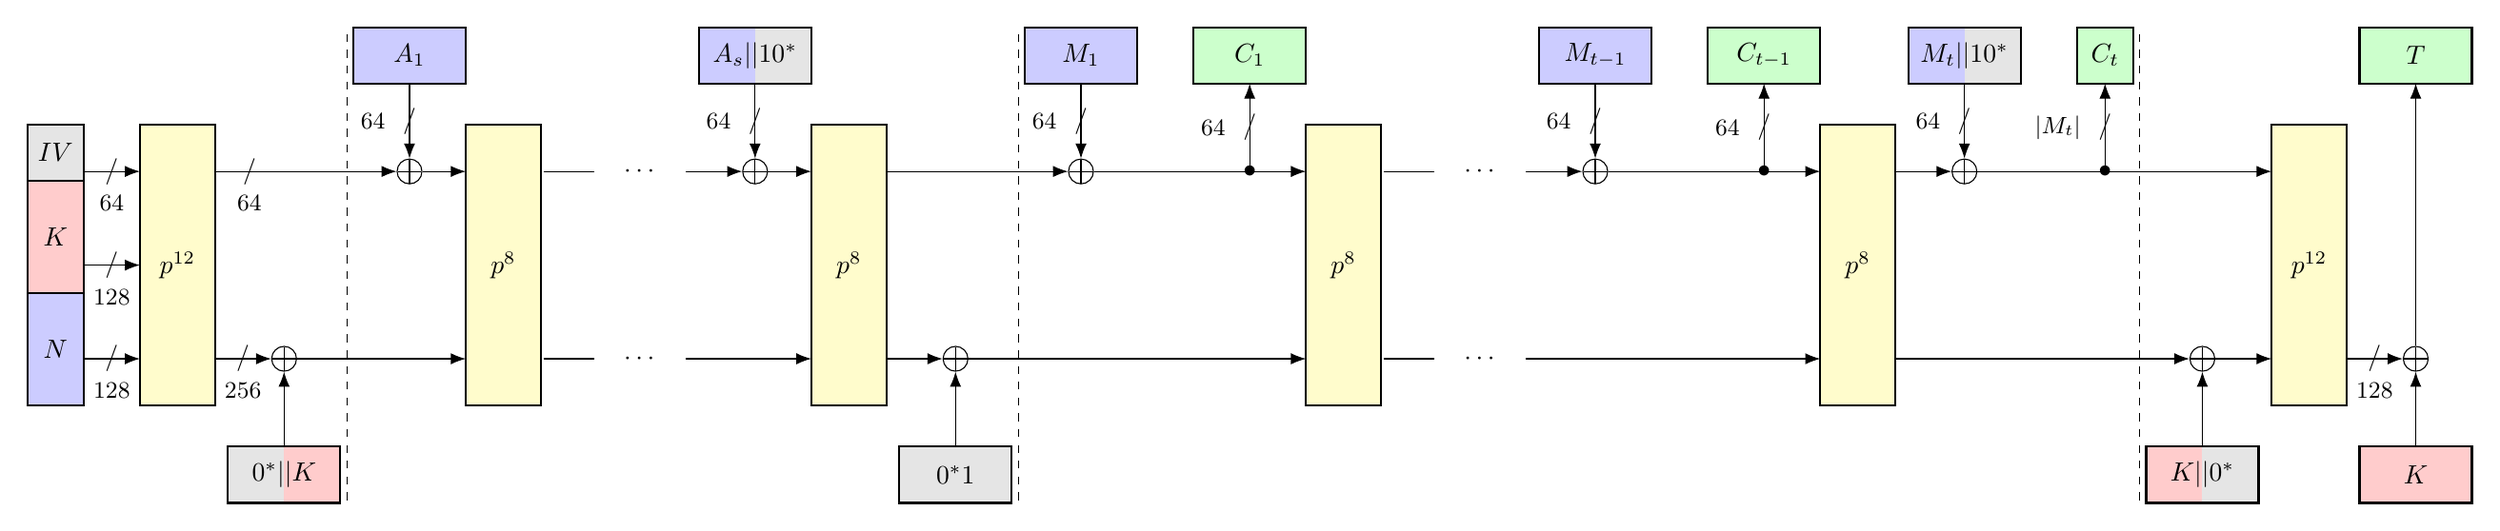
\begin{tikzpicture}[node distance = 1cm and 0.75cm]

% init
\node[AE_P, minimum height = 3.75cm] (pi) {$p^{12}$};

\node[AE_vert, fill = gray!20, left = of pi.north west, anchor = north east, minimum height = 0.75cm] (iv) {$IV$}; 

\node[AE_vert, fill = red!20, anchor = north] (k)  at (iv.south) {$K$}; 
\node[AE_vert, fill = blue!20, left = of pi.south west, anchor = south east] (n) {$N$}; 

\coordinate (helpsouth) at ($(pi.south east)!1/6!(pi.north east)$);
\coordinate (helpnorth) at ($(pi.south east)!5/6!(pi.north east)$);

\draw[-{Latex[length=2mm]}] (iv.east|-helpnorth) -> (helpnorth-|pi.west) node[midway] {$/$} node[midway, below=0.2cm] {\small $64$};
\draw[-{Latex[length=2mm]}] (k.east|-pi.west) -- (pi.west) node[midway] {$/$} node[midway, below=0.2cm] {\small $128$};
\draw[-{Latex[length=2mm]}] (n.east|-helpsouth) -- (helpsouth-|pi.west) node[midway] {$/$} node[midway, below=0.2cm] {\small $128$};

\node[XOR, right = of pi.east|-helpsouth] (xkinit) {};
\node[AE_key, anchor = west, below = of xkinit, path picture={
      \fill[gray!20] (path picture bounding box.north) rectangle (path picture bounding box.south west);
    }] (kinit) {$0^* || K$};

\draw[-{Latex[length=2mm]}] (pi.east|-helpsouth) -- (xkinit) node[midway] {$/$} node[midway, below=0.2cm] {\small $256$}; 
\draw[-{Latex[length=2mm]}] (kinit.north-|xkinit) -- (xkinit); 



% 1er tour AD

\node[XOR, right = of kinit.east|-helpnorth] (xa1) {};

\node[AE_msg, above = of xa1] (a1) {$A_1$};

\draw[-{Latex[length=2mm]}] (a1) -- (xa1) node[midway] {$/$} node[midway, left=0.2cm] {\small $64$};
\draw[line] (pi.east|-xa1) -- (helpnorth-|xkinit) node[midway] {$/$} node[midway, below=0.2cm] {\small $64$};
\draw[-{Latex[length=2mm]}] (pi.east|-xa1)  -- (xa1);


% 2er tour AD


\node[AE_P, minimum height = 3.75cm, right = of xa1|-pi] (pa1) {$p^{8}$};

\draw[-{Latex[length=2mm]}] (xkinit) -- (pa1.west|-xkinit);
\draw[-{Latex[length=2mm]}] (xa1) -- (pa1.west|-xa1);

\node[right = of pa1.east|-helpnorth, inner sep = 10pt] (cdotnortha) {$\cdots$};
\node[right = of pa1.east|-helpsouth, inner sep = 10pt] (cdotsoutha) {$\cdots$};

\node[XOR, right = of cdotnortha] (xa2) {};
\node[AE_msg, above = of xa2, path picture={
      \fill[gray!20] (path picture bounding box.north) rectangle (path picture bounding box.south east);
    }] (a2) {$A_{s}||10^*$};


\draw[line] (pa1.east|-cdotnortha) -- (cdotnortha);
\draw[line] (pa1.east|-cdotsoutha) -- (cdotsoutha);
\draw[-{Latex[length=2mm]}] (cdotnortha) -- (xa2);
\draw[-{Latex[length=2mm]}] (a2) -- (xa2) node[midway] {$/$} node[midway, left=0.2cm] {\small $64$};


% fin AD

\node[AE_P, minimum height = 3.75cm, right = of xa2|-pa1] (pa2) {$p^{8}$};

\node[XOR, right = of pa2.east|-helpsouth] (xdom) {};
\node[AE_key, fill = gray!20, below = of xdom] (dom) {$0^*1$};

\draw[-{Latex[length=2mm]}] (xa2) -- (pa2.west|-xa2);
\draw[-{Latex[length=2mm]}] (cdotsoutha) -- (pa2.west|-helpsouth);

\draw[-{Latex[length=2mm]}] (pa2.east|-xdom) -- (xdom);
\draw[-{Latex[length=2mm]}] (dom.north-|xdom) -- (xdom);



% 1er tour chiffrement

\node[XOR, right = of dom.east|-helpnorth] (x1) {};
\node[AE_msg, above = of x1] (m1) {$M_1$};
\node[AE_ctx, right = of m1] (c1) {$C_1$};

\draw[-{Latex[length=2mm]}] (pa2.east|-x1) -- (x1);
\draw[-{Latex[length=2mm]}] (m1) -- (x1) node[midway] {$/$} node[midway, left=0.2cm] {\small $64$};
\draw[-{Latex[length=2mm]}] (x1) -| (c1)node[near end] {$/$} node[near end, left=0.2cm] {\small $64$};

\node at (x1-|c1) {$\bullet$};

% 2e tour chiffrement

\node[AE_P, minimum height = 3.75cm, right = of c1|-pa2] (p1) {$p^{8}$};

\draw[-{Latex[length=2mm]}] (x1) -- (x1-|p1.west);
\draw[-{Latex[length=2mm]}] (xdom) -- (p1.west|-helpsouth);

\node[right = of p1.east|-helpnorth, inner sep = 10pt] (cdotnorth) {$\cdots$};
\node[right = of p1.east|-helpsouth, inner sep = 10pt] (cdotsouth) {$\cdots$};

\node[XOR, right = of cdotnorth] (x2) {};
\node[AE_msg, above = of x2] (m2) {$M_{t-1}$};
\node[AE_ctx, right = of m2] (c2) {$C_{t-1}$};


\draw[line] (p1.east|-cdotnorth) -- (cdotnorth);
\draw[line] (p1.east|-cdotsouth) -- (cdotsouth);

\draw[-{Latex[length=2mm]}] (cdotnorth) -- (x2);
\draw[-{Latex[length=2mm]}] (m2) -- (x2) node[midway] {$/$} node[midway, left=0.2cm] {\small $64$};
\draw[-{Latex[length=2mm]}] (x2) -| (c2) node[near end] {$/$} node[near end, left=0.2cm] {\small $64$};

\node at (x2-|c2) {$\bullet$};


% fin chiffrement

\node[AE_P, minimum height = 3.75cm, right = of c2|-p1] (p2) {$p^{8}$};

\draw[-{Latex[length=2mm]}] (x2) -- (x2-|p2.west);
\draw[-{Latex[length=2mm]}] (cdotsouth) -- (p2.west|-cdotsouth);

\node[XOR, right = of p2.east|-x1] (x3) {};
\node[AE_msg, above = of x3, path picture={
      \fill[gray!20] (path picture bounding box.north) rectangle (path picture bounding box.south east);
    }] (m3) {$M_{t}||10^*$};
\node[AE_ctx, right = of m3, text width = 0.75cm] (c3) {$C_{t}$};

\draw[-{Latex[length=2mm]}] (p2.east|-x3) -- (x3);
\draw[-{Latex[length=2mm]}] (m3) -- (x3) node[midway] {$/$} node[midway, left=0.2cm] {\small $64$};
\draw[-{Latex[length=2mm]}] (x3) -| (c3) node[near end] {$/$} node[near end, left=0.2cm] {\small $|M_t|$};

\node at (x3-|c3) {$\bullet$};


% finalisation

\node[XOR, right = of c3.east|-helpsouth] (xkf) {};

\node[AE_P, minimum height = 3.75cm, right = of xkf.east|-p2] (pf) {$p^{12}$};

\node[AE_key, below = of xkf, path picture={
      \fill[gray!20] (path picture bounding box.north) rectangle (path picture bounding box.south east);
    }] (kf) {$K||0^*$};

\draw[-{Latex[length=2mm]}] (x3) -- (x3-|pf.west);
\draw[-{Latex[length=2mm]}] (p2.east|-xkf) -- (xkf);
\draw[-{Latex[length=2mm]}] (xkf|-kf.north) -- (xkf);
\draw[-{Latex[length=2mm]}] (xkf) -- (xkf-|pf.west);

\node[XOR, right = of pf.east|-xkf] (xt) {};
\node[AE_key, below = of xt] (kt) {$K$};
\node[AE_tag] at (c3-|xt) (t) {$T$};

\draw[-{Latex[length=2mm]}] (pf.east|-xt) -- (xt) node[midway] {$/$} node[midway, below=0.2cm] {\small $128$};
\draw[-{Latex[length=2mm]}] (kt) -- (xt);
\draw[-{Latex[length=2mm]}] (xt) -- (t);


% separations

\coordinate (sepinit) at ($(kinit.east)!1/2!(a1.west)$);
\draw[line, dashed] (kinit.south-|sepinit) -- (a1.north-|sepinit);

\coordinate (sepa) at ($(dom.east)!1/2!(m1.west)$);
\draw[line, dashed] (dom.south-|sepa) -- (m1.north-|sepa);

\coordinate (sepf) at ($(c3.east)!1/2!(kf.west)$);
\draw[line, dashed] (kf.south-|sepf) -- (c3.north-|sepf);

\end{tikzpicture}
}
		\caption{Ascon Encryption process from \cite{cours_crypto}}
		\label{fig:enc}
	\end{figure}
	
	
	\section{Equations for linking the output of the S-box to the key} \label{equations}
	\begin{gather*}
		S_4^j = n_o^j \oplus n_1^j \oplus k_0^j \times (1 \oplus IV^j \oplus n_1^j)\\
		S _4^j =\left \{	
		\begin{array}{ll}
			k_0^j \times (1 \oplus IV^j) & if\ (n_0^j,n_1^j)=(0,0)\\
			k_0^j \times IV^j & if\ (n_0^j,n_1^j)=(1,1)\\
			1 \oplus k_0^j \times IV^j & if\ (n_0^j,n_1^j)=(0,1)\\
			1 \oplus k_0^j \times (1 \oplus IV^j) & if\ (n_0^j,n_1^j)=(1,0)\\
		\end{array}
		\right.
	\end{gather*}
	
	\noindent Then if $IV^j = 0$: 
	$$S _4^j =\left \{	
	\begin{array}{ll}
		k_0^j& if\ (n_0^j,n_1^j)=(0,0)\\
		0& if\ (n_0^j,n_1^j)=(1,1)\\
		1& if\ (n_0^j,n_1^j)=(0,1)\\
		1 \oplus k_0^j& if\ (n_0^j,n_1^j)=(1,0)\\
	\end{array}
	\right.$$
	
	\noindent Otherwise, if $IV^j = 1$:
	$$S _4^j =\left \{	
	\begin{array}{ll}
		0& if\ (n_0^j,n_1^j)=(0,0)\\
		k_0^j& if\ (n_0^j,n_1^j)=(1,1)\\
		1 \oplus k_0^j& if\ (n_0^j,n_1^j)=(0,1)\\
		1& if\ (n_0^j,n_1^j)=(1,0)\\
	\end{array}
	\right.$$
	
	
	\section{Complementary graphs}
	\begin{figure}[H]
		\centering
		\includegraphics[scale=0.3]{img_files/vertical_one_byte}
		\caption{Mutual information between power consumption and Hamming weight of the concatenation of the first bit of each of the word of $S$ and its value like \ref{vHW} but for random nonces}
		\label{vHW&val}
	\end{figure}
	
	\begin{figure}[H]
		\centering
		\includegraphics[scale=0.3]{img_files/HWalea}
		\caption{Mutual information between power consumption and vertical HW or random possible HW}
		\label{HWalea}
	\end{figure}
	
	\section{Main code} \lstinputlisting[language=C,style=Cstyle,caption=Implementation for ascon.c]{code_files/ascon.c}
	
	\lstinputlisting[language=C,style=Cstyle,caption=Implementation for ascon.h]{code_files/ascon.h}
	
	\lstinputlisting[language=C,style=Cstyle,caption=Implementation for permutation.c]{code_files/permutation.c}
	
	\lstinputlisting[language=C,style=Cstyle,caption=Implementation for permutation.h]{code_files/permutation.h}
	
	\lstinputlisting[language=C,style=Cstyle,caption=Implementation for main.c]{code_files/main.c}
	
	\lstinputlisting[language=Python,style=Cstyle,caption=Implementation for trace capture for the ChipWhisperer]{code_files/traces_sca.py}
	
	\lstinputlisting[style=CStyle, caption=Analysis in Julia of the traces following the established attack]{code_files/decryption_analysis_cpa.jl}
	
\end{document}
